\documentclass[12pt]{extarticle}

\usepackage{geometry}
\geometry{
a4paper,
total={170mm,257mm},
left=20mm,
top=20mm,
headheight=12pt
}

\usepackage[parfill]{parskip} % Activate to begin paragraphs with an empty line rather than an indent
\usepackage{graphicx}
\usepackage{amsmath, amssymb, amsthm}
\usepackage[font=small,labelfont=bf]{caption, subcaption}
\usepackage{setspace}\onehalfspacing
\usepackage[loose,nice]{units}
\usepackage{array}
\usepackage[super]{nth}
\usepackage{graphicx}
\usepackage{float}
\usepackage{varioref}
\usepackage[unicode=true,colorlinks=true,urlcolor=blue,citecolor=black,linkcolor=black]{hyperref}
\usepackage{cleveref}
\usepackage{subcaption}
\usepackage{mathtools}
\usepackage[all]{nowidow}
\usepackage{wrapfig}
\usepackage{pdfpages}
\usepackage{authblk}
\usepackage[utf8x]{inputenc}
\usepackage[english]{babel}
\usepackage{xcolor}
% appendix
\usepackage[title,page]{appendix}
\usepackage{chngcntr}
% unbreakable dashes
\usepackage[shortcuts]{extdash}
% footnotes
\renewcommand{\thefootnote}{\fnsymbol{footnote}}

% less space before sections 
% \titlespacing*{<command>}{<left>}{<before-sep>}{<after-sep>}
\usepackage{titlesec}
\titlespacing*{\section}
{0pt}{2ex plus 1ex minus .2ex}{2ex plus .2ex}
\titlespacing*{\subsection}
{0pt}{1ex plus 1ex minus .2ex}{1ex plus .2ex}
\titlespacing*{\paragraph}
{0pt}{1ex plus 1ex minus .2ex}{1ex plus .2ex}

%SetFonts
% newtxtext+newtxmath
\usepackage{newtxtext} %loads helv for ss, txtt for tt
\usepackage{amsmath}
\usepackage[bigdelims]{newtxmath}
\usepackage[T1]{fontenc}
\usepackage{textcomp}
%SetFonts

% Supplementary
% https://support.authorea.com/en-us/article/how-to-create-an-appendix-section-or-supplementary-information-1g25i5a/
\newcommand{\beginsupplement}{%
      	\setcounter{table}{0}
        \renewcommand{\thetable}{S\arabic{table}}%
        \setcounter{figure}{0}
        \renewcommand{\thefigure}{S\arabic{figure}}%
		\setcounter{equation}{0}
        \renewcommand{\theequation}{A\arabic{equation}}%
}
% NatBib
\usepackage[numbers,square,comma,sort]{natbib}
\bibliographystyle{vancouver}
\setcitestyle{numbers}
\renewcommand{\bibsection}{}
%\renewcommand{\bibfont}{\small}

% math stuff
\DeclareMathOperator*{\E}{{\rm I\kern-.3em E}}
\newcommand*{\tr}{^\intercal}
\let\vec\mathbf
\newcommand{\matrx}[1]{{\left[ \stackrel{}{#1}\right]}}
\newcommand{\diag}[1]{\mbox{diag}\matrx{#1}}
\newcommand{\goesto}{\rightarrow}
\newcommand{\dspfrac}[2]{\frac{\displaystyle #1}{\displaystyle #2} }
\newtheorem{theorem}{Theorem}
\newtheorem{corollary}{Corollary}
\newtheorem{lemma}{Lemma}
\newtheorem{remark}{Remark}
\newtheorem{result}{Result}
\renewcommand\qedsymbol{} % no square at end of proof
\newcommand{\cl}{\mathbf{L}}
\newcommand{\cj}{\mathbf{J}}
\newcommand{\ci}{I}

% line numbers
\usepackage[displaymath, mathlines]{lineno}
\renewcommand\linenumberfont{\normalfont\small\sffamily}
\linenumbers
\modulolinenumbers[2]

%%%%%%%%%%%%%%%%%%%%%%%%%%%%%%%%%%%%%%%%%%
% Title 
\title{Supplementary Figures for \\ Prestige bias in cultural evolutionary dynamics}

% Authors
\renewcommand\Affilfont{\small}

\author[1,2]{Saar Egozi}
\author[2,3,$\dagger$]{Yoav Ram}

\affil[1]{School of Computer Science, Reichman University, Herzliya, Israel}
\affil[2]{School of Zoology, Faculty of Life Sciences, Tel Aviv University, Tel Aviv, Israel}
\affil[3]{Sagol School of Neuroscience, Tel Aviv University, Tel Aviv, Israel}
\affil[$\dagger$]{Corresponding author: yoavram@tauex.tau.ac.il}

%%%%%%%%%%%%%%%%%%%%%%%%%%%%%%%%%%%%%%%%%%
\begin{document}
\maketitle

\beginsupplement % https://support.authorea.com/en-us/article/how-to-create-an-appendix-section-or-supplementary-information-1g25i5a/

\begin{figure}[h]
    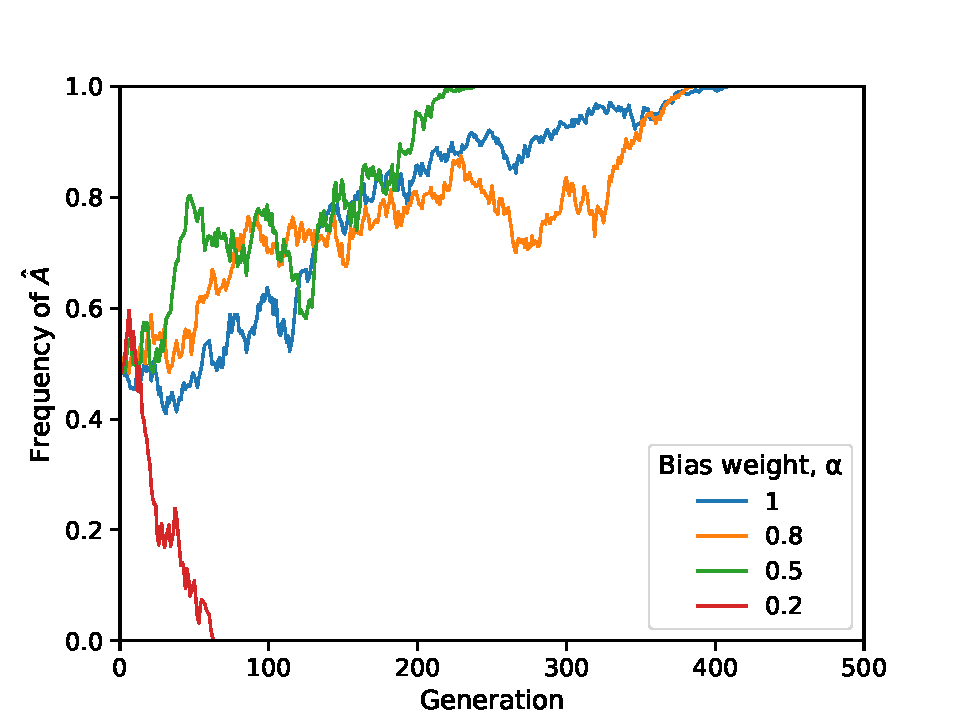
\includegraphics[width=1\linewidth]{timeseries.pdf}
  \caption{
  \textbf{Example dynamics of the dichotomous model with varying bias weight.}
  The dichotomous model is defined in eq.~11. Shown are full dynamics without DM or GBD approximations.
  Here, population size, $N=1,000$; ideal phenotype value, $\hat{A}=1$; success bias value, $\beta(A)=0.99$; initial phenotype frequencies are 50\%-50\%.
  }	
  \label{fig:timeseries}
\end{figure}


\begin{figure}[h]
    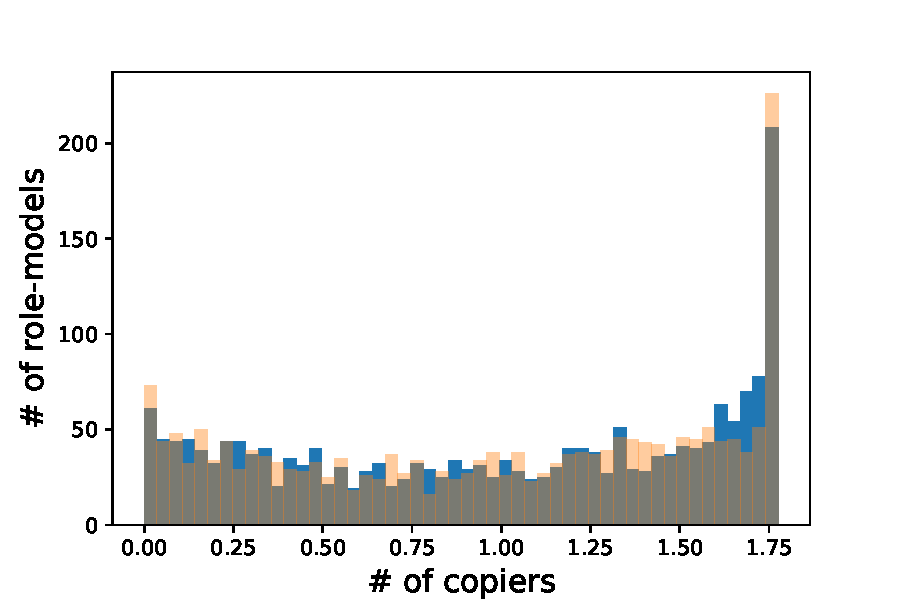
\includegraphics[width=0.7\linewidth]{GBD_validation.pdf}
  \caption{
  \textbf{Numerical validation of the GB approximation.}
  The approximation (orange) fits simulation results (blue) well when using 1,000 simulations. 
  Here, population size, $N=2,000$; bias weight, $\alpha=0.1$; {ideal} phenotype value, $\hat{A}=1$; role-model traits $\vec{A} \sim N(0,1)$; success bias value, $\beta(A)=0.956$.}	
  \label{fig:GBD}
\end{figure}


\begin{figure}[h]
    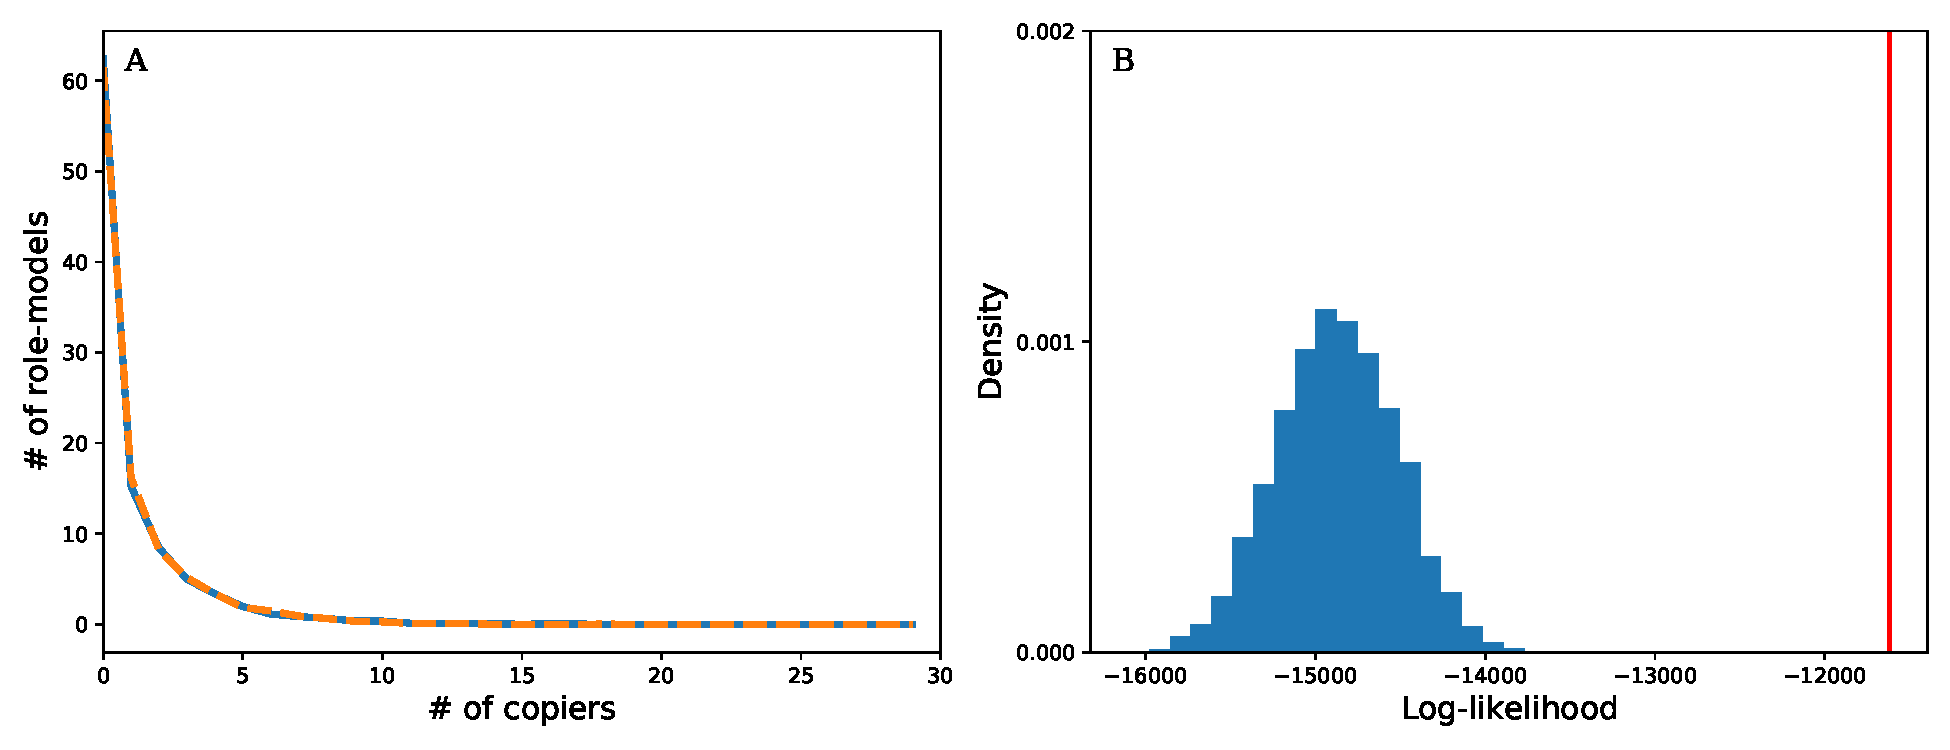
\includegraphics[width=\linewidth]{DM_validation.pdf}
  \caption{
  \textbf{Numerical validation of the DM approximation.}
  We performed computational simulations of the role-model choice process (eq.~10) and compared the distribution of the number of copiers to simulations when using the DMD approximation (corollary 2).
  \textbf{(A)} The difference between the DM distribution (orange) and the empirical distribution of the simulations (blue) is very small. 
  \textbf{(B)} The log-likelihood of the DMD for results of the simulations (red vertical line) is much higher {than} the log-likelihood of permutations of simulations (blue histogram).
  Here, population size, $N=100$; number of simulations, $m=100$; phenotype values, $\hat{A}=1$, $A \sim N(0,1)$; success-bias weight, $\alpha=0.5$.
  No estimation error or bias is applied, and traits are estimated and copied perfectly.}	
  \label{fig:DM_validation}
\end{figure}


\begin{figure}[h]
    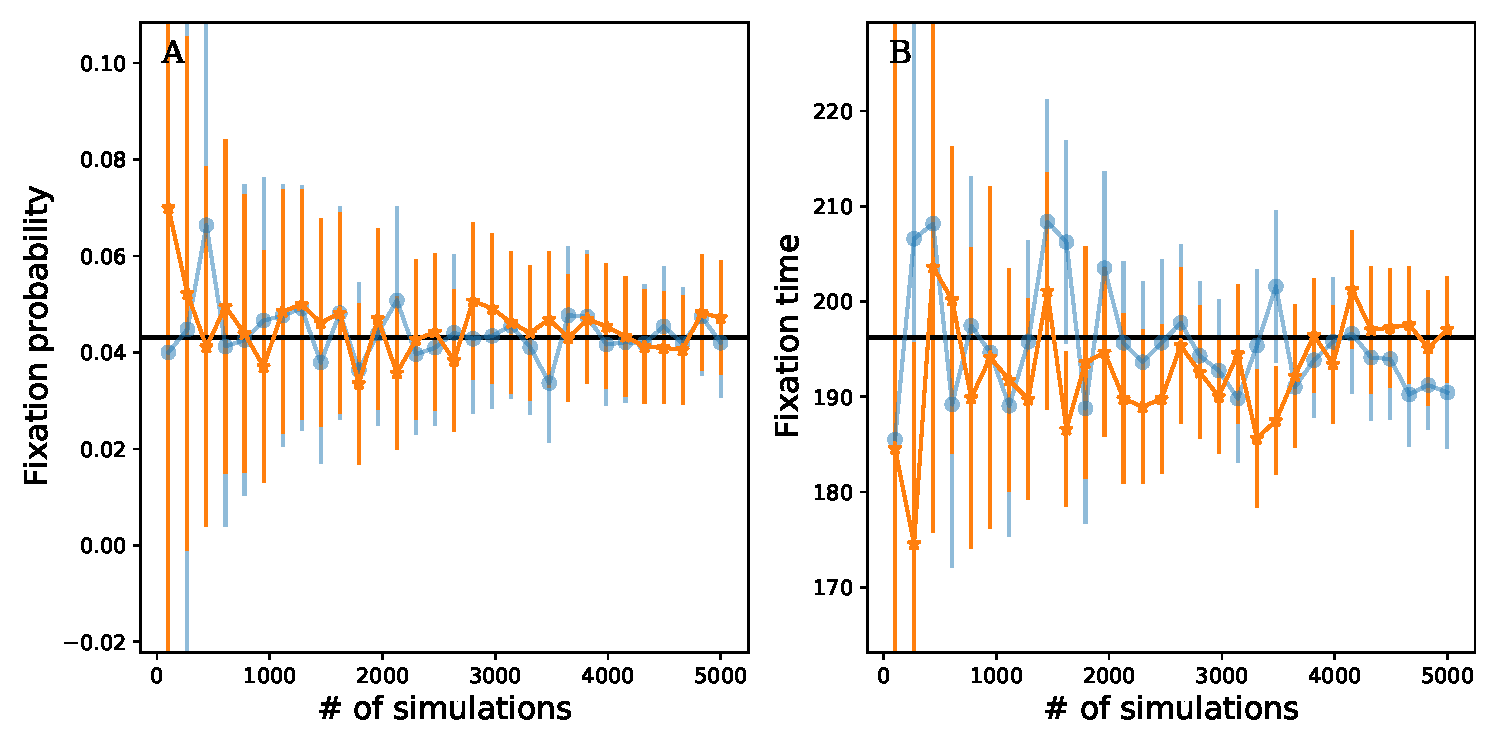
\includegraphics[width=\linewidth]{num_sims.pdf}
  \caption{
  \textbf{DMD approximation precision as function of number of simulations.}
  Our DMD approximation (orange) agrees with stochastic simulation results (blue) when using 1,000 or more simulations.
  Both fluctuate around the analytic fixation probability approximation (black; eq.~19).
  Markers are averages across simulations, error bars are 95\% confidence intervals.
  Here, population size, $N=1000$; success-bias weight, $\alpha=0.5$; phenotype values, $\hat{A}=1$, $A=0.7$; success-bias value, $\beta(A)=0.956$.}	
  \label{fig:num_sims}
\end{figure}


\begin{figure}
    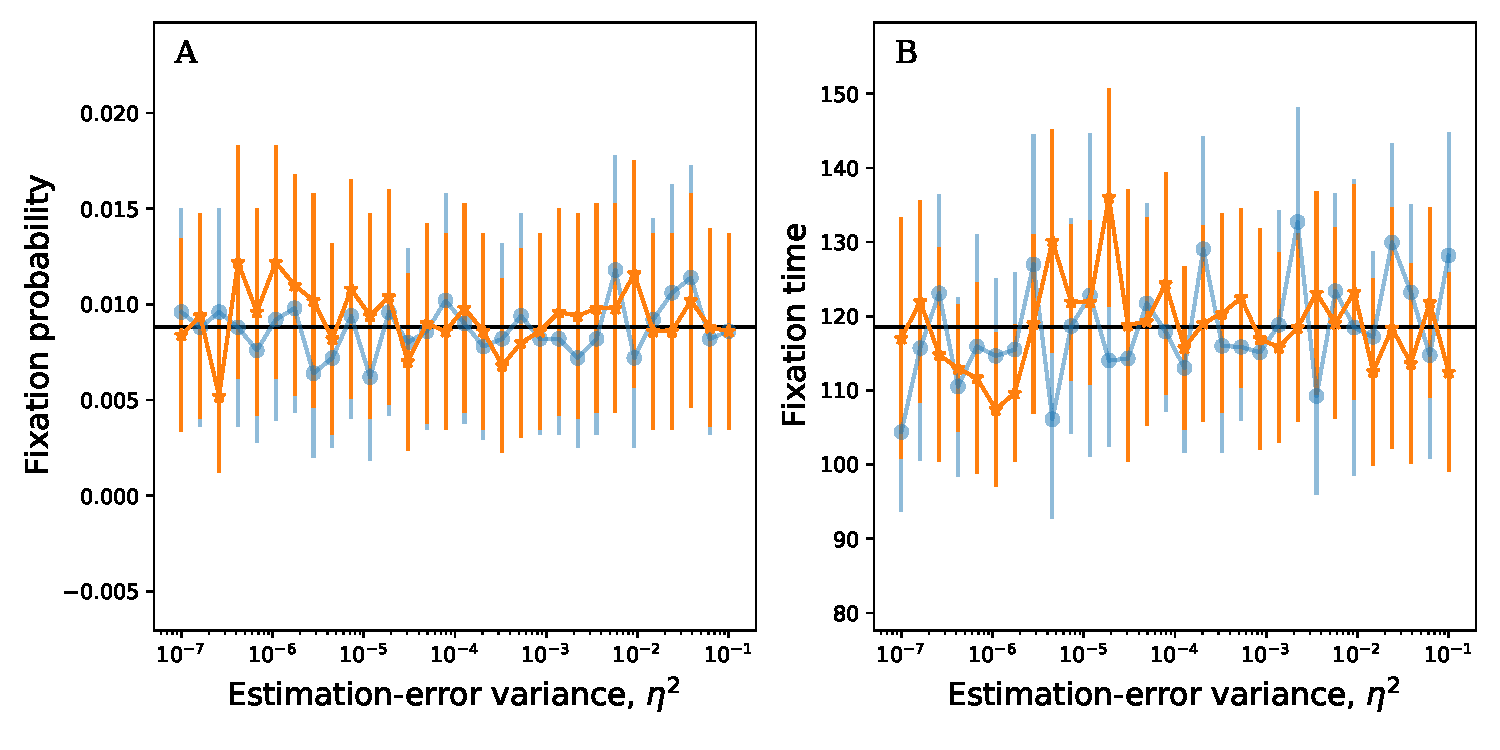
\includegraphics[width=\linewidth]{full_vs_dm_mutation.pdf}
  \caption{
  \textbf{Robustness of DMD approximations to success estimation error.}
  Both the DMD approximation (orange) and our approximation (black) agree with the stochastic simulations (blue), even with a high estimation error.
  Markers are averages across simulations, error bars are 95\% confidence intervals.
  5,000 simulations per data point; population size, $N=1000$; success-bias weight, $\alpha=0.1$; phenotype values, $\hat{A}=1$,$A=0.7$; bias strength parameter $J\sim N(1,\eta^2)$ where $\eta^2$ in on the x-axis.
  }	
  \label{fig:hetro_error}
\end{figure}


\begin{figure}
    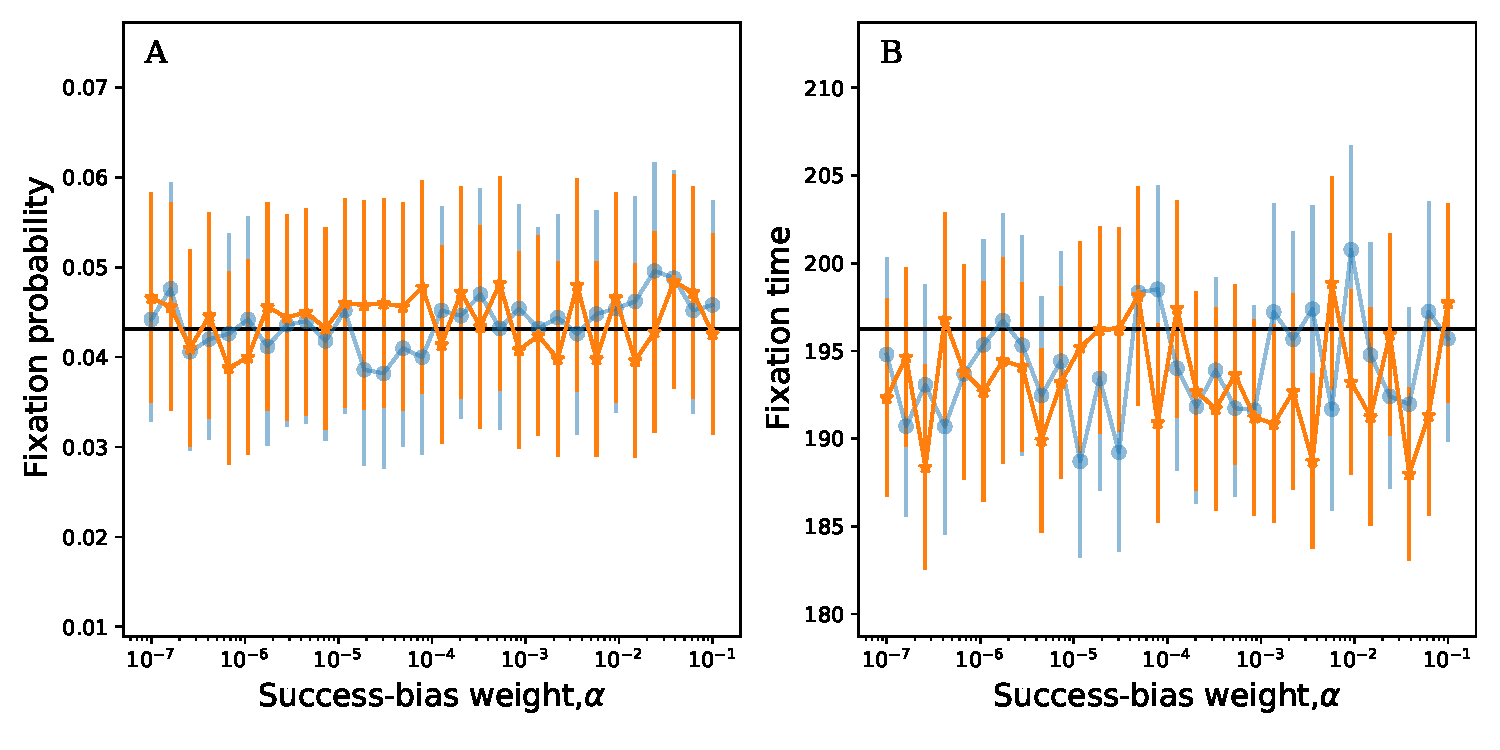
\includegraphics[width=\linewidth]{full_vs_dm_changing_alpha.pdf}
   \caption{\textbf{Robustness of DM approximations to variation in the bias weight $\alpha$.} 
   Fixation probability does not seem to be affected by variation in success bias weight between role-models.
    Thus, both the DM approximation (orange) and Kimura's equation (black line) have a good fit to results of stochastic simulations (blue).
   Markers for average across $5,000$ simulations, error bars are 95\% confidence intervals.
  Here, population size, $N=1000$; 
  success bias weight is normally distributed, $\alpha_j \sim N(0.5,\epsilon^2)$ where $10^{-7}\le \epsilon^2 \le 10^{-1}$; 
  phenotype values ,$\hat{A}=1$,$A=0.7$; success bias value, $\beta(A)=0.956$.}	
  \label{fig:hetro_alpha}
\end{figure}


\begin{figure}
	\centering
    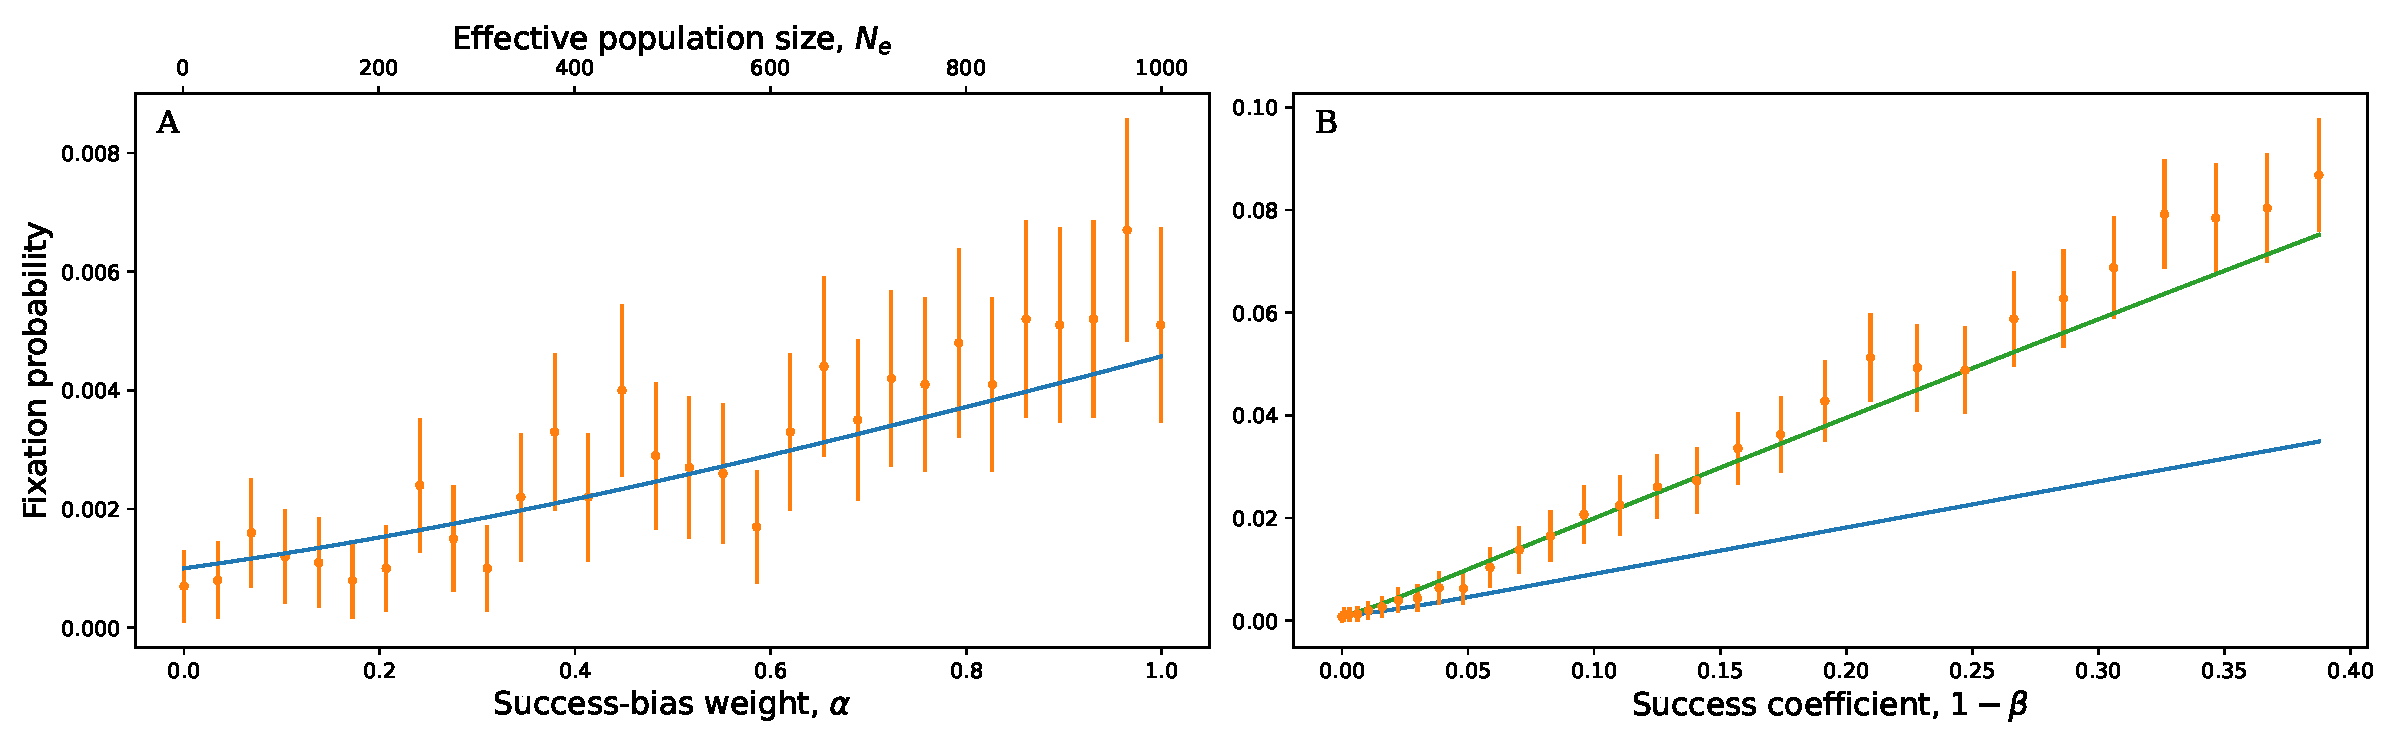
\includegraphics[width=\linewidth]{ch_env_k_large.pdf}
  \caption{\textbf{Fixation probability in a changing environment, $k>l$.}
\textbf{(A)} Fixation probability decreases with {the} success-bias weight (bottom x-axis) and effective population size (top x-axis). The approximation (blue; \cref{eq:ch_env}) agrees with simulation results (orange). 
\textbf{(B)} Fixation probability increases with the success coefficient, $\beta$.
When success bias is large ($1-\beta > 0.1$),  
simulation results (orange) are underestimated by the changing environment approximation (blue; eq.~23). With even larger success bias ($1-\beta > 0.35$), even the constant environment approximation (green; eq.~19) slightly underestimates simulation results, likely because the diffusion equation approximation assumes weak `selection'.
Markers show average of $10,000$ simulations, error bars show 75\% (panel A) and 95\% (panel B) confidence intervals.
Here, population size is $N=1,000$;
In panel A, $A=0.9$, $\hat{A}=1$ ($1-\beta=s=0.005$), $k=80$, and $l=20$;
In panel B, $0.01 < A< 0.99$, and $\hat{A}=1$, which determines $1-\beta$ via $\beta = \beta(A)/\beta(\hat{A})$ and eq.~5, $k=80$, and $l=20$, $\alpha=0.1$; 
}
\label{fig:ch_env_alpha_beta_k_large}
\end{figure}



\end{document}
